\chapter{Natural Language Processing}
\thispagestyle{fancy}
\label{chap:Natural Language Processing}

\noindent
Natürliche Sprache wird auch als menschliche Sprache bezeichnet und ist historisch gewachsen. Sie verfolgt orthographische und grammatikalische Regeln auf Grundlage eines sprachabhängigen Wortschatzes. Die Sprachwissenschaft, auch Linguistik genannt, untersucht natürliche Sprache mithilfe verschiedener Methoden. \ac{NLP} meint die maschinelle Verarbeitung natürlicher Sprache. Dabei werden Methoden der Linguistik unter anderem mit Methoden des Deep Learning verknüpft \cite[S.~1]{BIR09}. Nicht selten ist eine Spracherkennung vorgeschaltet. \ac{NLP} ist weiterhin in \ac{NLU} und \ac{NLG} zu untergliedern \cite[S.~27-28]{BIR09}. Diese Teilgebiete sind zugleich wesentliche Herausforderungen der \ac{ATS}.\\

\noindent
\ac{NLP}-Aufgaben sind oftmals als Optimierungsprobleme zu verstehen. Lösungen sind demnach nicht eindeutig, also im mathematischen Sinne analytisch nicht lösbar. Dies wird in Hinblick auf die \ac{ATS} deutlich, wenn man verschiedene Personen den gleichen Text zusammenfassen lässt. Zwar gleichen sich die als relevant identifizierten Informationen größtenteils, doch die Formulierungen sind mitunter sehr unterschiedlich. Folglich können auch mehrere Versionen korrekt sein.\\

\noindent
Natürliche Sprache bedarf hinsichtlich maschineller Verarbeitung einer geeigneten mathematischen Form. Hierfür werden nachfolgend verschiedene Vorverarbeitungsschritte sowie Word Embeddings und Deep Language Representations vorgestellt. Der Anspruch auf Vollständigkeit entfällt aufgrund der Mächtigkeit des \ac{NLP}, obgleich anknüpfende Inhalte bei Bedarf an den entsprechenden Stellen erläutert werden.
\newpage


\section{Vorverarbeitung}
\noindent
In nahezu allen Teilbereichen der Data Science stehen gewöhnlicherweise etliche Vorverarbeitungsschritte an, um die zu analysierenden Daten zu bereinigen, zu normalisieren und insgesamt in eine konsistente sowie geeignete Form zu bringen. Im \ac{NLP}-Kontext sind indes komplexere Vorverarbeitungsschritte erforderlich, um die Daten für die eingeforderte mathematische Form zu präparieren \cite[S.~86]{BIR09}. Eine Auswahl der in dieser Arbeit relevanten Schritte wird nachfolgend vorgestellt. In der Implementierung dieser chronologisch aufeinander folgenden Schritte spricht man auch von der \ac{NLP}-Pipeline.


\subsection{Textbereinigung}
\noindent
An erster Stelle der \ac{NLP}-Pipeline steht die Textbereinigung, welche sich bezüglich eingehender Sequenzen insbesondere auf Sonderzeichen, Interpunktion sowie Klein- und Großschreibung konzentriert. Dabei ist es mitunter bereits herausfordernd, entsprechende Textstellen als solche zu identifizieren. Anschließend sind oftmals normalisierende Maßnahmen anzuwenden. Üblich ist beispielsweise das Entfernen von Sonderzeichen oder auch das Erzwingen von Kleinschreibung in allen eingehenden Texten \cite[S.~107]{BIR09}. Weit verbreitet ist auch das Entfernen von Stoppwörtern. Dies sind Wörter, welche mutmaßlich der Allgemeinsprache zugehören, weshalb angenommen wird, dass sie keine entscheidende inhaltliche Bedeutung besitzen \cite[S.~5]{GAM16}. Hier lässt sich jedoch keine allgemeingültige Aussage treffen, da die tatsächlich erforderlichen Maßnahmen sowohl von den Eigenschaften der Eingangsdaten als auch von den Besonderheiten der verwendeten Modelle und den verfolgten Zielen abhängen. Dabei ist die Datenexploration wiederkehrend und alternierend mit der Anpassung der Vorverarbeitung auszuführen. Der Anwender sollte hierbei ein Gefühl für die Daten und deren Besonderheiten entwickeln. Zudem bedarf es einem tiefgründigen Verständnis der geplanten Aufgaben, um beurteilen zu können, welche Vorverarbeitungsschritte tatsächlich relevant sind.


\subsection{Textnormalisierung}
\noindent
In der weitergehenden Textnormalisierung wird sich vorrangig auf das Stemming und die Lemmatisierung konzentriert. Das Stemming führt eingehende Wörter auf ihre Grundformen zurück, indem bekannte Präfixe, Infixe und Suffixe eliminiert werden. Diese Grundformen sind nicht zwingend valide Wörter. Die Lemmatisierung hingegen berücksichtigt die wortspezifischen Bedeutungen, um etwaige Flexionen in Deckung zu bringen und somit die linguistisch korrekten Grundformen zu bilden. Flexionen sind durch Konjugationen, Deklinationen oder auch Komparationen entstanden und natürlicher Bestandteil einer Sprache. Hierfür sind Wortbildungsregeln und ein Wortschatz erforderlich. Letzterer indiziert die eingehenden Wörter anhand ihrer Lemmata und ordnet sie entsprechend zu \cite[S.~107-108]{BIR09}. Zwar ist die Lemmatisierung aufgrund des erforderlichen Kontextwissens durchaus komplexer als das Stemming, dafür sind ihre Ergebnisse erwartungsgemäß gehaltvoller. Ob und welche Methode zur Textnormalisierung herangezogen wird, hängt erneut von der anvisierten Aufgabe ab. Seien nun beispielhaft die Wörter \{\textit{spielen, spielst, spielte, gespielt}\} gegeben, dann reduziert der Stemmer diese Wörter auf die Grundform \textit{spiel}. Der Lemmatizer identifiziert hingegen die linguistisch korrekte Grundform \textit{spielen}.\\

\noindent
\ac{NLTK} ist eine forschungsorientierte Python-Bibliothek, die etliche \ac{NLP}-Module zur Verfügung stellt, darunter unter anderem verschiedenartige Stemmer \cite[S.~13-14]{BIR09}. Stemmer, welche die englische Sprache unterstützen, scheinen bereits sehr ausgereift zu sein. Stemmer, welche die deutsche Sprache unterstützen, sind nicht nur knapp, sondern bedürfen zudem weitergehenden Testschritten, um deren tatsächliche Eignung zu prüfen. Die Stemmer nltk.stem.cistem und nltk.stem.snowball eignen sich potenziell für einen Einsatz mit deutscher Sprache \cite{NLT20}.\\

\noindent
SpaCy ist eine eher praktisch orientierte Python-Bibliothek für verschiedenste \ac{NLP}-Aufgaben. Hinsichtlich der deutschen Sprache eignen sich hier insbesondere die verfügbaren Lemmatizer. Dabei kann der Anwender zwischen verschiedenen vortrainierten Modellen wählen. Eigenschaften wie Sprache, Größe und zugrundeliegende Trainingsdaten sind transparent dokumentiert \cite{SPA21}.\\

\noindent
Die Wahl geeigneter Stemmer und Lemmatizer obliegt dennoch den subjektiven Präferenzen des jeweiligen Entwicklers. In jedem Fall sind hinreichende Tests durchzuführen, um die einzelnen Module zu erproben sowie individuelle Vor- und Nachteile zu identifizieren. Mit fortschreitender Entwicklung beweisen sich möglicherweise auch andere aufstrebende Bibliotheken \cite[S.~108]{BIR09}.
\newpage


\subsection{Tokenisierung}
\noindent
In der Tokenisierung werden Texte in logisch zusammengehörige Token zerlegt. Texte bestehen aus Sequenzen, welche wiederum aus Symbolen, also etwa Zeichen, Zeichenketten oder auch Ziffern bestehen. Token sind indes als Einheiten der Wort- oder Satzebene zu verstehen \cite[S.~22-24]{MAN08}.\\

\noindent
Der einfachste Ansatz einer wortbasierten Tokenisierung besteht darin, den Text anhand von Leerzeichen und nicht-alphanumerischer Zeichen zu segmentieren. Dies ist jedoch nicht völlig obligatorisch und führt meist nicht zu einer verarbeitbaren Lösung, weshalb sprachabhängige Eigenarten berücksichtigt werden müssen. Typisch ist beispielsweise die Weiterbehandlung von vor- oder nachstehenden Klammern an den Token \cite[S.~109-111]{BIR09}.\\

\noindent
Ob weiterhin auch Interpunktion berücksichtigt oder verworfen werden soll, ist hinsichtlich der anvisierten \ac{NLP}-Aufgabe individuell zu entscheiden und zu erproben. Gleiches gilt für die Entscheidung, ob eingehende Texte roh oder vorverarbeitet hineingegeben werden.\\

\noindent
Sei nun ein Satz gegeben, welcher keiner Textbereinigung und keiner Textnormalisierung unterzogen wird. Eine Tokenisierung, welche die Eigenschaften der deutschen Sprache sowie Interpunktion hinreichend berücksichtigt, würde die in \autoref{pic:Tokenization} visualisierte Menge von Token generieren.

\begin{figure}[h!]
  \centering
  \fbox{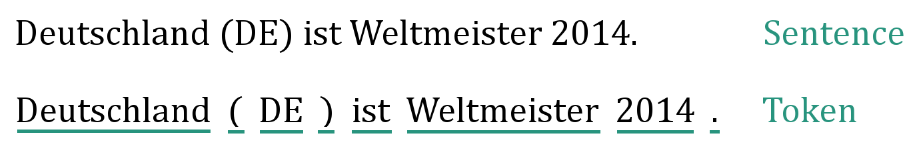
\includegraphics[width=0.6\linewidth]{./source/images/tokenization.png}}
  \caption{Tokenisierung eines beispielhaften Satzes.}
  \label{pic:Tokenization}
\end{figure}

\noindent
Die Arbeit mit Texten erfordert bekanntermaßen eine geeignete mathematische Form. Die zeichenbasierten Token der Texte werden daher in einem Wortschatz (engl. Vocabulary) mithilfe numerischer Indizes kodiert. Hier ist es möglich, die Anzahl eindeutiger Token zu identifizieren oder gar seltene Token aus praktischen Gründen zu entfernen \cite[S.~311-312]{ZHA20}.
\newpage

\noindent
Die Python-Bibliotheken \ac{NLTK} und SpaCy stellen entsprechende Tokenizer für eine möglichst schnelle Implementierung bereit. Beide sind überdies in einer für die deutsche Sprache ausgereiften Version verfügbar. Oftmals werden hierbei weitere Funktionalitäten mitgeliefert, darunter meist das Entfernen sprachbezogener Stoppwörter, die Lemmatisierung oder auch das Part-of-Speech-Tagging \cite[S.~111]{BIR09}.


\section{Word Embeddings}
\noindent
Word Embeddings überführen Texte in einen Vektorraum (engl. Vector Space), um Wörter syntaktisch, semantisch und insbesondere untereinander in Kontext zu bringen. Dabei wird ein Wortschatz benutzt, welcher die entsprechenden Vektoren, bestehend aus eindeutig kodierbaren ganzzahligen Werten, aufbaut \cite{KAR18}. Word Embeddings werden üblicherweise noch vor der Entwicklung der ursprünglichen \ac{NLP}-Aufgabe trainiert, weshalb ihnen ein unmittelbarer qualitativer Einfluss zugesprochen wird. Die entstehenden Modelle sind in der Folge schnell implementierbar. Weiterhin haben sie einen hohen skalierenden Effekt, da sie als Grundlage verschiedenster nachgelagerter \ac{NLP}-Aufgaben eingesetzt werden können \cite{NIT19}. Word Embeddings können durch verschiedene mehr oder minder komplexe Ansätze realisiert werden. Diese werden nachfolgend vorgestellt, wobei stets verdeutlicht wird, wie der entsprechende Vektorraum aufgebaut und in Kontext gebracht wird.


\subsection{One-Hot-Encoding}
\noindent
One-Hot-Encoding ist einer der einfachsten Ansätze, um Texte in einen Vektorraum einzubetten. Dabei werden allgemein kategorische Variablen in ein numerisches und somit mathematisch verarbeitbares Format gebracht \cite{KAR18}. Seien nun zwei gleichbedeutende Sätze gegeben. Eben jene Sätze sowie der entsprechende Wortschatz und die binär kodierten Vektoren sind in \autoref{pic:OneHotEncoding} ersichtlich. Die Vektoren sind hierbei als Matrix zusammengefasst, wobei die Zeilen und Spalten anhand der Anfangsbuchstaben der Wörter kenntlich gemacht sind.\\

\noindent
Versucht man nun, diese Vektoren in einem Vektorraum zu visualisieren, dann entspricht jeder Vektor einer eigenen Dimension. Dabei wird allerdings klar, dass keine dimensionsübergreifenden Projektionen existieren \cite{KAR18}. Dies bedeutet, dass die Wörter \textit{gutes} und \textit{schönes} genauso verschieden sind, wie die Wörter \textit{heute} und \textit{ist}. Dies ist offensichtlich falsch. One-Hot-Encoding ist dennoch als Grundlage zu verstehen, wobei etwaige Probleme innerhalb der nachfolgenden Ansätze weiterbehandelt werden.

\begin{figure}[h!]
  \centering
  \fbox{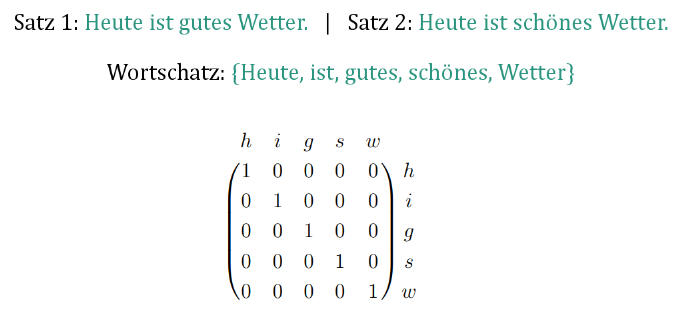
\includegraphics[width=0.65\linewidth]{./source/images/onehotencoding.png}}
  \caption{One Hot Encoding zwei beispielhafter Sätze.}
  \label{pic:OneHotEncoding}
\end{figure}


\subsection{Bag-of-Words}
\noindent
Text

\url{https://towardsdatascience.com/introduction-to-word-embedding-and-word2vec-652d0c2060fa}

\subsection{Word2Vec}
\noindent
Text

-> auf Basis von BOW und Skip-Gram

\subsection{Byte-Pair-Encoding}
\noindent
Text

\subsection{GloVe}
\noindent
Text


-> Word Embeddings in den Kontext des Language Modeling, d.h. Language Models einordnen (siehe Leveraging ...), ggf. bei den Deep Language Representations nach deren Definition aufgreifen

-> Keyword Network generieren, bestenfalls mit eigenem Modell, welches auf den eigenen Korpora basiert

-> Beschreibung im Kapitel der Encoder-Decoder-Architekturen unbedingt mit den jetzt neu gewonnenen Informationen aktualisieren


\section{Deep Language Representations}
Text

\subsection{BERT}
\noindent
Text

\subsection{ELMo}
\noindent
Text

\subsection{GPT}
\noindent
Text


Notizen:
\begin{itemize}
	\item Deep Language Models
	\item BERT als Encoder \& Decoder nutzen, Architekturen und TL dementsprechend aufgreifen (S. 1 in YAN19), bspw. als Encoder oder/ und Decoder verwenden, siehe ROT20 auf S. 2 rechts und S. 6 unten, Encoder zur NLU und Decoder zur NLG, d.h. BERT oder andere Transformer als vortrainiertes multilinguales Modell für Encoder/ Decoder nutzen, Ausblick auf Adaption von EN->DE: Fine-Tuning der Modelle, verschiedene Experimente, aber dazu im späteren Kapitel mehr, BERT ist außerdem austauschbar, durch sowohl größere als auch kleinere Modelle, Multilingualität architektonisch ergründen, erwähnen, dass diese Modelle die Encoder oder auch Decoder ersetzen können, hierzu populäre Ansätze wie \cite{ROT20}, Trainingsvorgehensweise von BERT und ELMo beschreiben, wie im Forschungsstand bereits erwähnt, konnten diese vortrainierten Language Models die NLU-Welt revolutionieren, wie viele Parameter wurden genutzt? Verschiedene Modelle vergleichen, bspw. das Notebook \url{https://colab.research.google.com/drive/1WIk2bxglElfZewOHboPFNj8H44_VAyKE?usp=sharing#scrollTo=4M2uzGLV9a_O} unter "Analysis" referenzieren, jeweils maximale Token-Länge oder verschieden trainierte Versionen hervorheben, ggf. LongFormer als Encoder benutzen
	\item BERT vs. Alternativen: \url{https://towardsdatascience.com/bert-roberta-distilbert-xlnet-which-one-to-use-3d5ab82ba5f8}
	\item ELMo
	\item GPT
	\item Transfer Learning mit BERT hier sinnvoll, sodass das Modell die Sprache nicht in einer bestimmten Domain oder mit zu wenigen Texten neu erlernen muss, TL durch Encoder, Decoder etc. auf jeden Fall hier aufgreifen
	\item BERT zunächst in Englisch nutzen, weil SOTA, ggf. Grafik aus Oli's VL integrieren, irgendwie in Abstractive Summarization Pipelines integrieren
	\item BERT ist auch multilingual, d.h. englisches Modell mit deutschem Fine-Tuning vermutlich sogar brauchbar
	\item Modell beschreiben, d.h. Datensätze und Parametrisierung, SOTA für verschiedene NLP-Tasks, von Kapazitäten profitieren, hat viel Kontextwissen, Fine-Tuning für eigenes Problem, d.h. domainspezifisch o.ä.
	\item Am besten direkt ein vortrainiertes Transformer-Modell nutzen (extra für Summarization-Tasks), BERT und RL bspw. in der Pipeline integrieren, Ziel wäre dann: Verbesserung im Score erzielen
	\item BERT vielleicht durch andere (teils bessere und neuere) Transformer ersetzen? Transformer in NLP recherchieren, LSTM als veraltet bezeichnen
\end{itemize}

Notizen:
\begin{itemize}
	\item Quelle: \cite{NIT19}
	\item Transfer Learning with German BERT? \url{https://deepset.ai/german-bert} -> Modell muss die deutsche Sprache nicht alleine und von neu  mit den Trainingsdaten lernen, sondern erhält einen großen Vorsprung, BERT ist Modell, welches der Transformer-Architektur nachkommt, d.h. Transformer sind bestimmte Architekturen, eventuell hiermit die Struktur dieses Kapitels überarbeiten, hier für vor allem aus meinem privaten Verzeichnis das Paper "Pre-Training of Deep Bidirectional Transformers for Language Understanding using BERT" nutzen
	\item GLoVe-Embeddings nutzen, weil TF-IDF etc. nicht den Kontext eines Satzes betrachten
	\item Supervised Learning nutzen, aber es ist eventuell nicht genug, hier kommt bspw. Transfer Learning mit BERT zur Abhilfe, zudem bspw. semi-supervised Learning mit Auto-Encoders? Self-supervised Training
	\item Siehe Abstract im Exposé
\end{itemize}
